\documentclass[12pt]{article}

\usepackage{amssymb,amsmath,amsfonts,bbm,bm,dcolumn,booktabs,eurosym,geometry,ulem,graphicx,color,xcolor,setspace,sectsty,comment,float,caption,subfigure,array,hyperref}
\usepackage{xurl}
\usepackage[font=bf]{caption}
\usepackage[bottom]{footmisc}

\hypersetup{
    colorlinks,
    linkcolor={black},
    citecolor={blue!35!black},
    urlcolor={blue!35!black}
}

\geometry{left=1.0in,right=1.0in,top=1.0in,bottom=1.0in}

\begin{document}
\title{Development Economics Problem Set 3}
\author{Steven VanOmmeren\thanks{A complete replication package of this project is available at \url{https://github.com/svanomm/development-econ/}.}}
\date{\today}
\maketitle

\doublespacing
\noindent

\begin{enumerate}
    \item \textbf{Show a scatter plot between output per worker and capital per worker. Instead of using the dots try to use the country codes in your chart similar to Figure 1 and Figure 2 in the paper.}
    \begin{figure}[H]
        \centering
        \caption{Scatter plot of output per worker vs. capital per worker}
        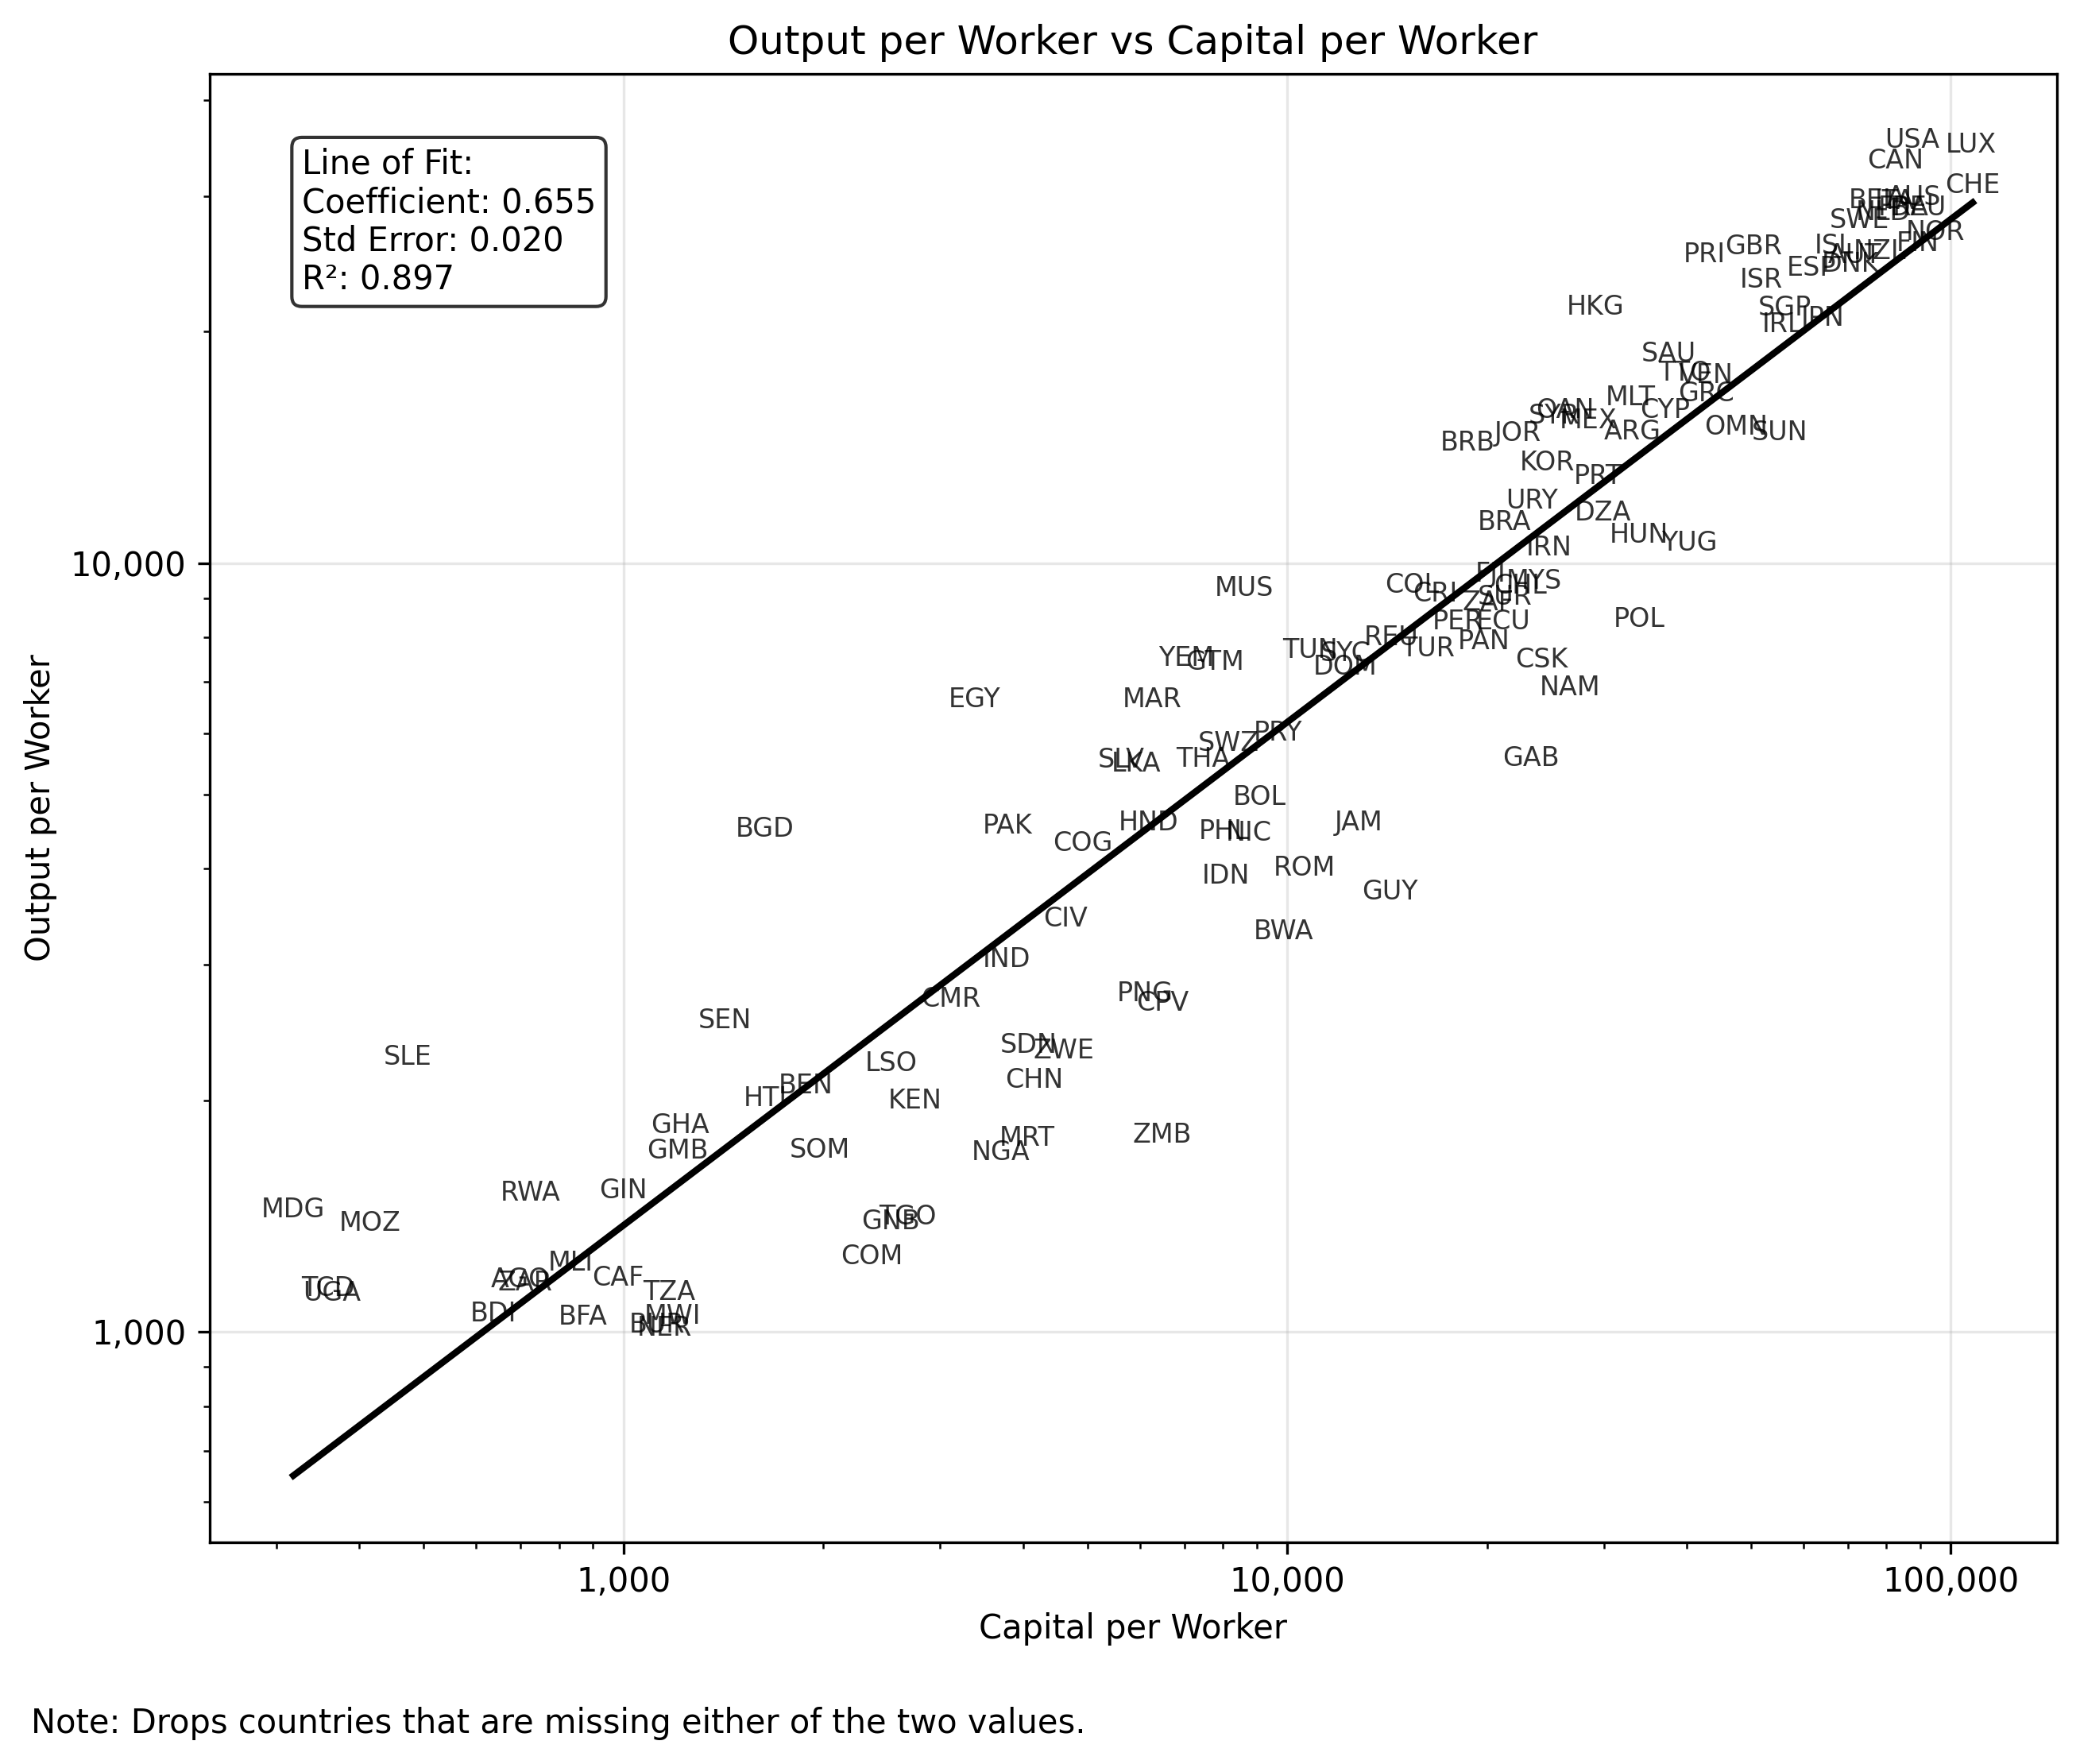
\includegraphics[width=0.8\textwidth]{output_vs_capital_scatter.png}
        \label{fig:scatter_output_capital}
    \end{figure}

    \item \textbf{Regress log output per worker on log capital per worker. Interpret your coefficients.}
    
    \begin{center}
\begin{tabular}{lclc}
\toprule
\textbf{Dep. Variable:}    &     hjlogyl      & \textbf{  R-squared:         } &    0.897  \\
\textbf{Model:}            &       OLS        & \textbf{  Adj. R-squared:    } &    0.896  \\
\textbf{Method:}           &  Least Squares   & \textbf{  F-statistic:       } &    1091.  \\
\textbf{Date:}             & Tue, 22 Jul 2025 & \textbf{  Prob (F-statistic):} & 1.31e-63  \\
\textbf{Time:}             &     12:59:44     & \textbf{  Log-Likelihood:    } &  -44.710  \\
\textbf{No. Observations:} &         127      & \textbf{  AIC:               } &    93.42  \\
\textbf{Df Residuals:}     &         125      & \textbf{  BIC:               } &    99.11  \\
\textbf{Df Model:}         &           1      & \textbf{                     } &           \\
\textbf{Covariance Type:}  &    nonrobust     & \textbf{                     } &           \\
\bottomrule
\end{tabular}
%\caption{OLS Regression Results}
\end{center}
    \begin{center}
\begin{tabular}{lcccccc}
\toprule
                 & \textbf{coef} & \textbf{std err} & \textbf{t} & \textbf{P$> |$t$|$} & \textbf{[0.025} & \textbf{0.975]}  \\
\midrule
\textbf{const}   &       2.7048  &        0.186     &    14.540  &         0.000        &        2.337    &        3.073     \\
\textbf{hjlogkl} &       0.6545  &        0.020     &    33.034  &         0.000        &        0.615    &        0.694     \\
\bottomrule
\end{tabular}
\end{center}

    The constant coefficient of 2.7048 means that if the log-capital per worker was equal to 0 for a country, then output per worker would be approximately \$14.95 (since $e^{2.7048} \approx 14.95$). The coefficient of log-capital per worker is 0.6545, which implies that a 1\% increase in capital per worker is associated with a 0.65\% increase in output per worker, on average. Because this is a log-log regression, the model measures the elasticity of output per worker with respect to capital per worker.
\\\\
    It also worth regressing output per worker on log of \textit{human} capital per worker, rather than physical capital:
    \begin{center}
\begin{tabular}{lclc}
\toprule
\textbf{Dep. Variable:}    &     hjlogyl      & \textbf{  R-squared:         } &    0.637  \\
\textbf{Model:}            &       OLS        & \textbf{  Adj. R-squared:    } &    0.634  \\
\textbf{Method:}           &  Least Squares   & \textbf{  F-statistic:       } &    219.5  \\
\textbf{Date:}             & Tue, 22 Jul 2025 & \textbf{  Prob (F-statistic):} & 2.69e-29  \\
\textbf{Time:}             &     12:59:44     & \textbf{  Log-Likelihood:    } &  -124.81  \\
\textbf{No. Observations:} &         127      & \textbf{  AIC:               } &    253.6  \\
\textbf{Df Residuals:}     &         125      & \textbf{  BIC:               } &    259.3  \\
\textbf{Df Model:}         &           1      & \textbf{                     } &           \\
\textbf{Covariance Type:}  &    nonrobust     & \textbf{                     } &           \\
\bottomrule
\end{tabular}
%\caption{OLS Regression Results}
\end{center}
    \begin{center}
\begin{tabular}{lcccccc}
\toprule
                 & \textbf{coef} & \textbf{std err} & \textbf{t} & \textbf{P$> |$t$|$} & \textbf{[0.025} & \textbf{0.975]}  \\
\midrule
\textbf{const}   &       7.0263  &        0.131     &    53.691  &         0.000        &        6.767    &        7.285     \\
\textbf{hjloghl} &       2.9709  &        0.201     &    14.816  &         0.000        &        2.574    &        3.368     \\
\bottomrule
\end{tabular}
\end{center}
    This regression shows that a 1\% increase in human capital per worker (e.g. additional education) is associated with a 2.97\% increase in output per worker. It also predicts that a country with no human capital (i.e. no education) would output an average of \$1,125.86 per worker ($e^{7.0263}$).

    \item \textbf{Measure Total Factor Productivity for this modified equation to the best of your ability.}
    
    I calculated TFP by rearranging Hall-Jones equation 3 using the log-terms, since that is what the data came with:
    \begin{align*}
    \log(y_i) &= \log\left(\frac{K_i}{Y_i}^{\alpha/(1-\alpha)}h_iA_i\right) \\
    &= \log\left(\frac{K_i}{Y_i}^{\alpha/(1-\alpha)}\right) + \log(h_i) + \log(A_i) \\
    &= \frac{\alpha}{1-\alpha}\log\left(\frac{K_i}{Y_i}\right) + \log(h_i) + \log(A_i) \\
    \log(A_i) &= \log(y_i) - \frac{\alpha}{1-\alpha}\log\left(\frac{K_i}{Y_i}\right) - \log(h_i) \\
    A_i &= \exp(\log(y_i) - \frac{\alpha}{1-\alpha}\log\left(\frac{K_i}{Y_i}\right) - \log(h_i))
    \end{align*}

    After calculating TFP, I then recreated Hall-Jones' Table 1, which shows the TFP relative to the United States. Note that the USA's value of TFP is 6815.126, so you can recover the value of TFP for each country by multiplying its relative TFP by 6815.126.

    \begin{table}[H]
\caption*{
{\large Productivity Calculations: Ratios to U.S. Values}
} 

\fontsize{12.0pt}{14.4pt}\selectfont

\begin{tabular*}{\linewidth}{@{\extracolsep{\fill}}lrrrr}
\toprule
Country & $Y/L$ & $(K/Y)^{\alpha/(1-\alpha)}$ & $H/L$ & A \\ 
\midrule\addlinespace[2.5pt]
U.S.A. & 1.000 & 1.000 & 1.000 & 1.000 \\
Canada & 0.941 & 1.002 & 0.908 & 1.034 \\
Italy & 0.834 & 1.063 & 0.650 & 1.207 \\
Germany, West & 0.818 & 1.118 & 0.802 & 0.912 \\
France & 0.818 & 1.091 & 0.666 & 1.126 \\
U.K. & 0.727 & 0.891 & 0.808 & 1.011 \\
Hong Kong & 0.608 & 0.741 & 0.735 & 1.115 \\
Singapore & 0.606 & 1.031 & 0.545 & 1.078 \\
Japan & 0.587 & 1.119 & 0.797 & 0.658 \\
Mexico & 0.433 & 0.868 & 0.538 & 0.926 \\
Argentina & 0.418 & 0.953 & 0.676 & 0.648 \\
U.S.S.R. & 0.417 & 1.231 & 0.724 & 0.468 \\
India & 0.086 & 0.709 & 0.454 & 0.267 \\
China & 0.060 & 0.891 & 0.632 & 0.106 \\
Kenya & 0.056 & 0.747 & 0.457 & 0.165 \\
Zaire & 0.033 & 0.499 & 0.408 & 0.160 \\
\bottomrule
\end{tabular*}
\begin{minipage}{\linewidth}
The elements of this table are the empirical counterparts to the components of equation (3), all measured as ratios to the U. S. values. That is, the first column of data is the product of the other three columns.\\
\end{minipage}
\end{table}

\end{enumerate}
\end{document}